\subsection[Proceso Interno 11: Procesar Datos]{Proceso Interno 11: Procesar Datos para Visualización}

\subsubsection{Objetivo del Proceso}
El propósito principal de la actividad ``Procesar Datos para Visualización'' es transformar y formatear los datos brutos del estado del sistema gravitacional, recolectados en el proceso ``Recolectar Datos'', para que sean compatibles y óptimos para la biblioteca o herramienta gráfica específica utilizada en la visualización. Esta actividad asegura que los datos estén en el formato adecuado y contengan solo la información relevante para generar gráficos como trayectorias 2D/3D o gráficos de energía, soportando la representación visual del comportamiento dinámico en el contexto de la simulación de dos cuerpos.

\subsubsection{Entradas Principales}
\begin{itemize}
    \item \textbf{Estructura \texttt{VisualizationState}}: Una estructura de datos (por ejemplo, un diccionario o objeto) que contiene la instantánea del sistema en un instante de visualización, incluyendo:
    \begin{itemize}
        \item Tiempo ($t$).
        \item Masas (\texttt{masas[]}).
        \item Posiciones (\texttt{posiciones[][]: } $\mathbf{r} = [x, y, z]$ por partícula).
        \item Velocidades (\texttt{velocidades[][]: } $\mathbf{v} = [v_x, v_y, v_z]$ por partícula, si se recolectaron).
        \item Metadatos opcionales (por ejemplo, nombres, colores, tamaños).
    \end{itemize}
    \item \textbf{Configuración de Visualización}:\ Información que define el tipo de gráfico a generar (por ejemplo, trayectoria 2D XY, trayectoria 3D, gráfico de energía vs\. tiempo) y parámetros de transformación, como:
    \begin{itemize}
        \item Límites de la ventana gráfica (por ejemplo, $x_{\text{min}}$, $x_{\text{max}}$, $y_{\text{min}}$, $y_{\text{max}}$).
        \item Factores de escala ($scale\_factor$) y traslación ($offset$).
        \item Requerimientos de proyección (por ejemplo, de 3D a 2D).
    \end{itemize}
\end{itemize}

\subsubsection{Sub-pasos Secuenciales}
Este apartado es proporcionado para profundizar y describir de forma textual cada paso contenido dentro del diagrama del proceso descrito en la figura~\ref{fig:process_diagram11}
\subsubsection*{1. Recibir Datos Recolectados}
\begin{itemize}
    \item La actividad recibe la estructura \texttt{VisualizationState} con los datos brutos del estado del sistema en el instante de visualización.
\end{itemize}

\subsubsection*{2. Verificación de Configuración}
\begin{itemize}
    \item \textbf{Leer Configuración de Visualización}: Se accede a la configuración de visualización para determinar:
    \begin{itemize}
        \item El tipo de gráfico (por ejemplo, trayectoria 2D, trayectoria 3D, energía vs.\ tiempo).
        \item Parámetros de transformación (escala, traslación, proyección).
        \item Límites y escalas de la ventana gráfica.
    \end{itemize}
    \item \textbf{Determinar Tipo de Gráfico}: Se identifica el tipo de gráfico especificado:
    \begin{itemize}
        \item Trayectoria 2D/3D:\ Configura el procesamiento para extraer coordenadas espaciales.
        \item Energía vs. Tiempo: Configura el procesamiento para incluir cálculos de energía.
        \item Otro: Configura el procesamiento según los requerimientos específicos del gráfico.
    \end{itemize}
\end{itemize}

\subsubsection*{3. Transformación de Coordenadas (Condicional)}
\begin{itemize}
    \item \textbf{Verificar Requerimiento de Transformación}: Se evalúa si las coordenadas físicas en \texttt{VisualizationState.posiciones} (potencialmente a gran escala) necesitan transformarse para adaptarse a la ventana gráfica o al formato de la biblioteca gráfica.
    \item \textbf{Si se requiere transformación}:
    \begin{itemize}
        \item \textbf{Inicializar Arrays}: Se crean arrays para almacenar las coordenadas transformadas.
        \item \textbf{Bucle por Partícula}: Para cada partícula:
        \begin{itemize}
            \item \textbf{Escalado}: Se aplica un factor de escala para mapear las coordenadas físicas a la escala gráfica:
            \[
            \mathbf{r}_{\text{scaled}} = (\mathbf{r}_{\text{original}} - \mathbf{r}_{\text{min}}) \times scale\_factor
            \]
            donde $\mathbf{r}_{\text{min}}$ y $scale\_factor$ provienen de la configuración.
            \item \textbf{Traslación}: Se aplica un desplazamiento para centrar las coordenadas en la ventana gráfica:
            \[
            \mathbf{r}_{\text{transformed}} = \mathbf{r}_{\text{scaled}} + offset
            \]
        \end{itemize}
        \item \textbf{Proyección (Si Aplica)}: Se evalúa si es necesaria una proyección de 3D a 2D (por ejemplo, para gráficos 2D).
        \begin{itemize}
            \item Si se requiere: Se aplica una matriz de proyección $\mathbf{P}$:
            \[
            \mathbf{r}_{\text{2D}} = \mathbf{P} \times \mathbf{r}_{\text{transformed}}
            \]
            donde $\mathbf{P}$ es la matriz de proyección definida por la configuración.
            \item Si no se requiere: Se mantienen las coordenadas transformadas sin proyección.
        \end{itemize}
        \item El bucle continúa hasta procesar todas las partículas.
    \end{itemize}
    \item \textbf{Si no se requiere transformación}: Se mantienen las coordenadas originales ($\mathbf{r}_{\text{transformed}} = \mathbf{r}_{\text{original}}$).
\end{itemize}

\subsubsection*{4. Selección de Datos Relevantes}
\begin{itemize}
    \item \textbf{Iniciar Selección}: Se identifican los datos necesarios según el tipo de gráfico especificado.
    \item \textbf{Según Tipo de Gráfico}:
    \begin{itemize}
        \item Trayectoria 2D:\ Se extraen las componentes $x$ e $y$ de las posiciones transformadas, almacenándolas en arrays como \texttt{x\_coords[]} y \texttt{y\_coords[]}.
        \item Trayectoria 3D:\ Se extraen las componentes $x$, $y$, y $z$, almacenándolas en \texttt{x\_coords[]}, \texttt{y\_coords[]}, y \texttt{z\_coords[]}.
        \item Energía vs. Tiempo: Se extraen el tiempo ($t$), masas ($m$), posiciones ($\mathbf{r}$), y velocidades ($\mathbf{v}$, si disponibles) para cálculos posteriores de energía.
        \item Otro: Se extraen los componentes relevantes según la configuración específica del gráfico.
    \end{itemize}
    \item Los datos seleccionados se almacenan para el siguiente paso.
\end{itemize}

\subsubsection*{5. Cálculos Derivados (Condicional)}
\begin{itemize}
    \item \textbf{Verificar Requerimiento de Cálculos}: Se evalúa si el tipo de gráfico requiere cálculos derivados (por ejemplo, energía o momento angular).
    \item \textbf{Si se requieren cálculos}:
    \begin{itemize}
        \item \textbf{Energía}: Se calculan:
        \begin{itemize}
            \item Energía cinética:
            \[
            E_k = \sum_{i} (0.5 \times m_i \times |\mathbf{v}_i|^2)
            \]
            \item Energía potencial:
            \[
            E_p = -G \sum_{i < j} \frac{m_i m_j}{|\mathbf{r}_i - \mathbf{r}_j|}
            \]
            \item Energía total:
            \[
            E_{\text{total}} = E_k + E_p
            \]
        \end{itemize}
        \item \textbf{Momento Angular}: Se calcula el momento angular total:
        \[
        \mathbf{L} = \sum_{i} m_i (\mathbf{r}_i \times \mathbf{v}_i)
        \]
        \item \textbf{Otros Cálculos}: Se realizan cálculos específicos según la configuración (por ejemplo, distancias relativas o velocidades relativas).
    \end{itemize}
    \item \textbf{Si no se requieren cálculos}: Se omiten los cálculos derivados, manteniendo solo los datos seleccionados.
\end{itemize}

\subsubsection*{6. Formateo para API Gráfica}
\begin{itemize}
    \item \textbf{Iniciar Formateo}: Se prepara la conversión de los datos seleccionados y derivados al formato requerido por la biblioteca gráfica (por ejemplo, \texttt{Matplotlib}, \texttt{Pygame}, \texttt{Plotly}).
    \item \textbf{Identificar Formato Requerido}: Se determina el formato esperado por la API:\
    \begin{itemize}
        \item Listas Separadas: Crear arrays individuales por eje (por ejemplo, \texttt{x\_list = [x1, x2, \ldots]}, \texttt{y\_list = [y1, y2, \ldots]}).
        \item Lista de Tuplas: Crear una lista de puntos (por ejemplo, \texttt{points = [(x1, y1), (x2, y2), \ldots]}).
        \item Arrays NumPy: Convertir los datos a arrays \texttt{NumPy} (por ejemplo, \texttt{X = np.array~([x1, x2, \ldots])}, \texttt{Y = np.array~([y1, y2, \ldots])}).
        \item Diccionario/Objeto: Crear una estructura con metadatos (por ejemplo, \texttt{data = \{`x': [x1, x2, \ldots], `y': [y1, y2, \ldots], `tipo': `scatter'\}}).
    \end{itemize}
    \item Los datos se convierten al formato seleccionado, incluyendo cualquier valor derivado (como energías).
\end{itemize}

\subsubsection*{7. Finalizar Estructura de Datos}
\begin{itemize}
    \item Se completa la estructura de datos formateada, que contiene los datos transformados, seleccionados, y posiblemente derivados, en el formato exacto requerido por la biblioteca gráfica.
\end{itemize}

\subsubsection*{8. Pasar Datos Formateados}
\begin{itemize}
    \item La estructura de datos formateada se envía al proceso ``Generar Gráficos'' del pipeline de visualización, donde se utilizará para renderizar la representación gráfica.
\end{itemize}

\subsubsection{Lógica Interna y Decisiones}
\begin{itemize}
    \item \textbf{Tipo de Gráfico}: La selección del tipo de gráfico (trayectoria 2D, 3D, energía, otro) determina las ramas de procesamiento, afectando la selección de datos y los cálculos derivados.
    \item \textbf{Transformación de Coordenadas}: La decisión de transformar coordenadas depende de la configuración de visualización. Si es necesaria, se aplican escalado, traslación, y proyección condicionalmente (por ejemplo, proyección 3D a 2D solo para gráficos 2D).
    \item \textbf{Cálculos Derivados}: La necesidad de cálculos como energía o momento angular introduce una bifurcación. Gráficos como trayectorias omiten estos cálculos, mientras que gráficos de energía los requieren.
    \item \textbf{Formato de la API}: La elección del formato (listas, tuplas, \texttt{NumPy}, diccionario) depende de la biblioteca gráfica, permitiendo flexibilidad para diferentes herramientas.
    \item \textbf{Manejo de Errores Implícito}: Errores como datos inválidos (por ejemplo, divisiones por cero en el cálculo de energía potencial) son manejados por validaciones previas o excepciones en la biblioteca gráfica, fuera del alcance directo de esta actividad.
\end{itemize}

\subsubsection{Manejo de Datos Específico}
\begin{itemize}
    \item \textbf{Datos de Entrada}:
    \begin{itemize}
        \item Estructura \texttt{VisualizationState} con tiempo, masas, posiciones, velocidades (si aplica), y metadatos.
        \item Configuración de visualización (tipo de gráfico, parámetros de transformación).
    \end{itemize}
    \item \textbf{Datos Intermedios}:
    \begin{itemize}
        \item Coordenadas transformadas (escaladas, trasladadas, proyectadas: $\mathbf{r}_{\text{transformed}}, \mathbf{r}_{\text{2D}}$).
        \item Subconjuntos de datos seleccionados (por ejemplo, \texttt{x\_coords}, \texttt{y\_coords}).
        \item Valores derivados (por ejemplo, energía cinética $E_k$, potencial $E_p$, total $E_{\text{total}}$, momento angular $\mathbf{L}$).
    \end{itemize}
    \item \textbf{Datos de Salida}:
    \begin{itemize}
        \item Estructura de datos formateada (por ejemplo, \texttt{x\_list}, \texttt{y\_list}, arrays \texttt{NumPy}, o diccionario) específica para la API de la biblioteca gráfica.
    \end{itemize}
\end{itemize}

\subsubsection{Salidas Principales}
\begin{itemize}
    \item \textbf{Datos Formateados para Visualización}: Una estructura de datos que contiene los datos del estado del sistema, seleccionados, transformados, y formateados según los requisitos de la biblioteca gráfica, lista para ser utilizada directamente en el proceso ``Generar Gráficos''.
\end{itemize}

\subsubsection{Interacciones Internas}
\begin{itemize}
    \item \textbf{Con el Proceso Anterior}: Recibe la estructura \texttt{VisualizationState} del proceso ``Recolectar Datos''.
    \item \textbf{Con la Configuración de Visualización}: Lee los parámetros de configuración para determinar el tipo de gráfico, transformaciones, y formato de salida.
    \item \textbf{Con Cálculos Matemáticos}: Realiza operaciones como escalado, traslación, proyección, y cálculos de energía o momento angular, según sea necesario.
    \item \textbf{Con el Pipeline de Visualización}: Transfiere los datos formateados al proceso ``Generar Gráficos'', integrándose en el flujo de renderización gráfica.
\end{itemize}
\newpage
\subsubsection{Diagrama del Proceso}
\begin{figure}[H]
    \centering
    \adjustbox{max width=\textwidth, max height=0.9\textheight}{%
    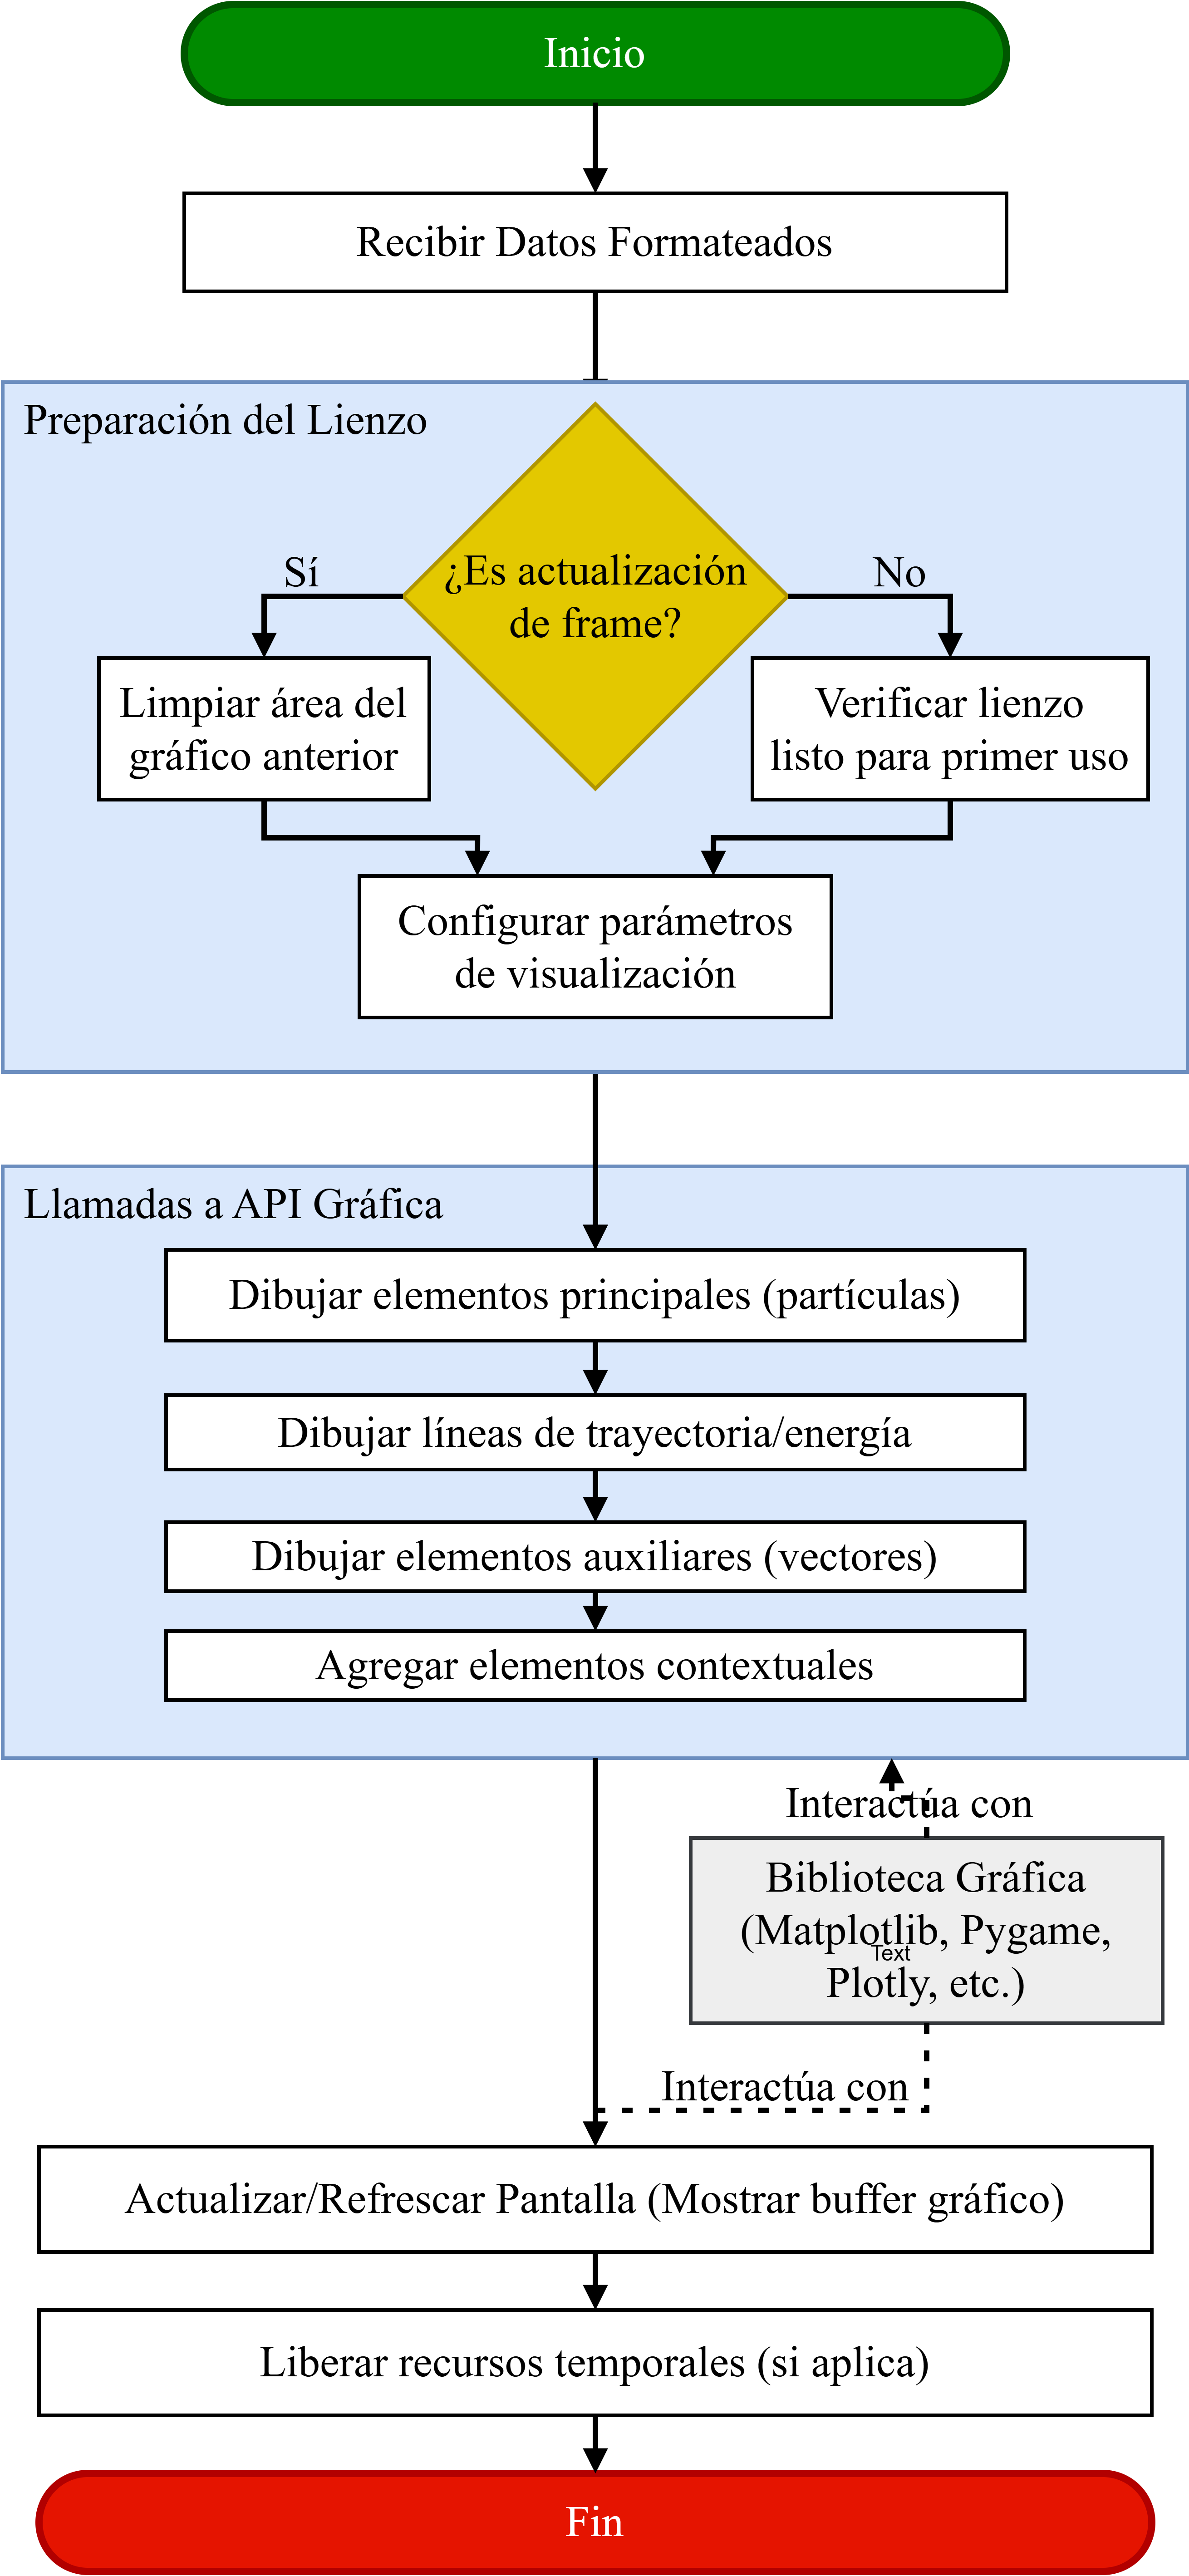
\includegraphics{img/Analisis/DiagramaProcesos/DiagramaProceso12_GenerarGrafico.png}
    }
    \caption{Diagrama de Proceso Interno 12: Generar Gráfico}%
    \label{fig:process_diagram12}
\end{figure}
\newpage